\documentclass[
  shownotes,
  xcolor={svgnames},
  hyperref={colorlinks,citecolor=DarkBlue,linkcolor=andesred,urlcolor=DarkBlue}
  , aspectratio=169]{beamer}
\usepackage{animate}
\usepackage{amsmath}
\usepackage{amsfonts}
\usepackage{amssymb}
\usepackage{pifont}
\usepackage{mathpazo}
%\usepackage{xcolor}
\usepackage{multimedia}
\usepackage{fancybox}
\usepackage[para]{threeparttable}
\usepackage{multirow}
\setcounter{MaxMatrixCols}{30}
\usepackage{subcaption}
\usepackage{graphicx}
\usepackage{lscape}
\usepackage[compatibility=false,font=small]{caption}
\usepackage{booktabs}
\usepackage{ragged2e}
\usepackage{chronosys}
\usepackage{appendixnumberbeamer}
\usepackage{animate}
\setbeamertemplate{caption}[numbered]
\usepackage{color}
%\usepackage{times}
\usepackage{tikz}
\usetikzlibrary{arrows}
\usepackage{comment} %to comment
%% BibTeX settings
\usepackage{natbib}
\bibliographystyle{apalike}
\bibpunct{(}{)}{,}{a}{,}{,}
\setbeamertemplate{bibliography item}{[\theenumiv]}

% Defines columns for bespoke tables
\usepackage{array}
\newcolumntype{L}[1]{>{\raggedright\let\newline\\\arraybackslash\hspace{0pt}}m{#1}}
\newcolumntype{C}[1]{>{\centering\let\newline\\\arraybackslash\hspace{0pt}}m{#1}}
\newcolumntype{R}[1]{>{\raggedleft\let\newline\\\arraybackslash\hspace{0pt}}m{#1}}


\usepackage{xfrac}


\usepackage{multicol}
\setlength{\columnsep}{0.5cm}

% Theme and colors
\usetheme{Boadilla}

% I define a custom pallete
\definecolor{andesred}{HTML}{1B175E}
\definecolor{andesyellow}{HTML}{ffff00}

% Other options
\providecommand{\U}[1]{\protect\rule{.1in}{.1in}}
\usefonttheme{serif}
\setbeamertemplate{itemize items}[default]
\setbeamertemplate{enumerate items}[square]
\setbeamertemplate{section in toc}[circle]


\definecolor{mybackground}{HTML}{1B175E}
\definecolor{myforeground}{HTML}{0000A0}

\setbeamercolor{normal text}{fg=black,bg=white}
\setbeamercolor{alerted text}{fg=andesred}
\setbeamercolor{example text}{fg=black}

\setbeamercolor{background canvas}{fg=myforeground, bg=white}
\setbeamercolor{background}{fg=myforeground, bg=mybackground}
\setbeamercolor{palette tertiary}{fg=myforeground,bg=mybackground}

\setbeamercolor{palette primary}{fg=black, bg=white}
\setbeamercolor{palette secondary}{fg=black, bg=white!10!andesyellow}
\setbeamercolor{palette tertiary}{fg=black, bg=white}


\setbeamercolor{frametitle}{fg=black}
\setbeamercolor{title}{fg=black}
\setbeamercolor{block title}{fg=andesred}
\setbeamercolor{itemize item}{fg=andesred}
\setbeamercolor{itemize subitem}{fg=andesred}
\setbeamercolor{itemize subsubitem}{fg=andesred}
\setbeamercolor{enumerate item}{fg=andesred}
\setbeamercolor{item projected}{bg=gray!30!white,fg=andesred}
\setbeamercolor{enumerate subitem}{fg=andesred}
\setbeamercolor{section number projected}{bg=gray!30!white,fg=andesred}
\setbeamercolor{section in toc}{fg=andesred}
\setbeamercolor{caption name}{fg=andesred}
\setbeamercolor{button}{bg=gray!30!white,fg=andesred}
\setbeamercolor{title in head/foot}{fg=andesred}



\usepackage{fancyvrb}
\newcommand{\VerbBar}{|}
\newcommand{\VERB}{\Verb[commandchars=\\\{\}]}
\DefineVerbatimEnvironment{Highlighting}{Verbatim}{commandchars=\\\{\}}
% Add ',fontsize=\small' for more characters per line
\usepackage{framed}
\definecolor{shadecolor}{RGB}{248,248,248}
\newenvironment{Shaded}{\begin{snugshade}}{\end{snugshade}}
\newcommand{\AlertTok}[1]{\textcolor[rgb]{0.94,0.16,0.16}{#1}}
\newcommand{\AnnotationTok}[1]{\textcolor[rgb]{0.56,0.35,0.01}{\textbf{\textit{#1}}}}
\newcommand{\AttributeTok}[1]{\textcolor[rgb]{0.77,0.63,0.00}{#1}}
\newcommand{\BaseNTok}[1]{\textcolor[rgb]{0.00,0.00,0.81}{#1}}
\newcommand{\BuiltInTok}[1]{#1}
\newcommand{\CharTok}[1]{\textcolor[rgb]{0.31,0.60,0.02}{#1}}
\newcommand{\CommentTok}[1]{\textcolor[rgb]{0.56,0.35,0.01}{\textit{#1}}}
\newcommand{\CommentVarTok}[1]{\textcolor[rgb]{0.56,0.35,0.01}{\textbf{\textit{#1}}}}
\newcommand{\ConstantTok}[1]{\textcolor[rgb]{0.00,0.00,0.00}{#1}}
\newcommand{\ControlFlowTok}[1]{\textcolor[rgb]{0.13,0.29,0.53}{\textbf{#1}}}
\newcommand{\DataTypeTok}[1]{\textcolor[rgb]{0.13,0.29,0.53}{#1}}
\newcommand{\DecValTok}[1]{\textcolor[rgb]{0.00,0.00,0.81}{#1}}
\newcommand{\DocumentationTok}[1]{\textcolor[rgb]{0.56,0.35,0.01}{\textbf{\textit{#1}}}}
\newcommand{\ErrorTok}[1]{\textcolor[rgb]{0.64,0.00,0.00}{\textbf{#1}}}
\newcommand{\ExtensionTok}[1]{#1}
\newcommand{\FloatTok}[1]{\textcolor[rgb]{0.00,0.00,0.81}{#1}}
\newcommand{\FunctionTok}[1]{\textcolor[rgb]{0.00,0.00,0.00}{#1}}
\newcommand{\ImportTok}[1]{#1}
\newcommand{\InformationTok}[1]{\textcolor[rgb]{0.56,0.35,0.01}{\textbf{\textit{#1}}}}
\newcommand{\KeywordTok}[1]{\textcolor[rgb]{0.13,0.29,0.53}{\textbf{#1}}}
\newcommand{\NormalTok}[1]{#1}
\newcommand{\OperatorTok}[1]{\textcolor[rgb]{0.81,0.36,0.00}{\textbf{#1}}}
\newcommand{\OtherTok}[1]{\textcolor[rgb]{0.56,0.35,0.01}{#1}}
\newcommand{\PreprocessorTok}[1]{\textcolor[rgb]{0.56,0.35,0.01}{\textit{#1}}}
\newcommand{\RegionMarkerTok}[1]{#1}
\newcommand{\SpecialCharTok}[1]{\textcolor[rgb]{0.00,0.00,0.00}{#1}}
\newcommand{\SpecialStringTok}[1]{\textcolor[rgb]{0.31,0.60,0.02}{#1}}
\newcommand{\StringTok}[1]{\textcolor[rgb]{0.31,0.60,0.02}{#1}}
\newcommand{\VariableTok}[1]{\textcolor[rgb]{0.00,0.00,0.00}{#1}}
\newcommand{\VerbatimStringTok}[1]{\textcolor[rgb]{0.31,0.60,0.02}{#1}}
\newcommand{\WarningTok}[1]{\textcolor[rgb]{0.56,0.35,0.01}{\textbf{\textit{#1}}}}
\usepackage{graphicx}
\makeatletter

\makeatother




\AtBeginSection[]
{
    \begin{frame}
        \frametitle{Agenda}
        \tableofcontents[currentsection]
    \end{frame}
}



\AtBeginSubsection[]
{
    \begin{frame}
        \frametitle{Agenda}
        \tableofcontents[currentsubsection]
    \end{frame}
}




%%%%%%%%%%%%%%% BEGINS DOCUMENT %%%%%%%%%%%%%%%%%%


\begin{document}


\title{Árboles (CARTs), Bagging and Random Forests}
\subtitle{Big Data y Machine Learning para Economía Aplicada}
\date{}

\author[Sarmiento-Barbieri]{Ignacio Sarmiento-Barbieri}
\institute[Uniandes]{Universidad de los Andes}


\begin{frame}[noframenumbering]
\maketitle
\end{frame}


%----------------------------------------------------------------------% 


\begin{frame}
\frametitle{Motivación: Recap}


\begin{itemize}
    \item Queremos predecir:

    \begin{align}
    Price=f(structural\,attributes,amenities,...)
    \end{align}
    \medskip
    \begin{itemize}
      \item Podemos aplicar linear regression,
    \end{itemize}
    \begin{align}
    Price=\beta_0 + \beta_1 Habitaciones + \beta_2 DCBD + u
    \end{align}
  \medskip

  \item Aplicar OLS a este problema requiere tomar algunas decisiones.
  \end{itemize}
\end{frame}
%----------------------------------------------------------------------% 
\begin{frame}[fragile]
\frametitle{Motivación: Recap}



\begin{figure}[H] \centering
            \captionsetup{justification=centering}
              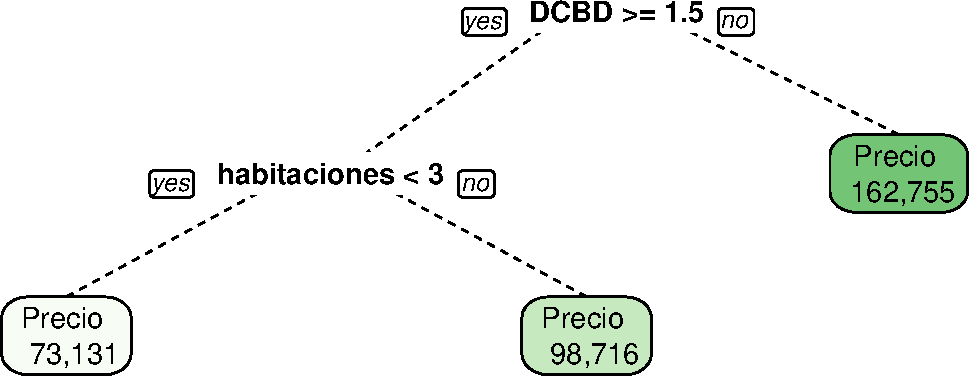
\includegraphics[scale=0.4]{figures/trees.pdf}                           
 \end{figure}

\end{frame}


%----------------------------------------------------------------------%
\begin{frame}[fragile]
\frametitle{Motivación: Recap}
\begin{figure}[H] \centering
  \centering
  
\includegraphics[scale=0.35]{figures/baticomputer_meme.jpg}
  \\
  \tiny photo from \url{https://www.dailydot.com/parsec/batman-1966-labels-tumblr-twitter-vine/}
\end{figure}

\end{frame}


%----------------------------------------------------------------------%
\section{Bagging }
%----------------------------------------------------------------------%
\begin{frame}[fragile]
\frametitle{Bagging}

\begin{itemize}
  \item Problema con CART: pocos robustos.
  \medskip
   \item Podemos mejorar mucho el rendimiento mediante la agregación 
   \medskip
     \item Idea: la varianza del promedio es menor que la de una sola predicción.
\end{itemize}

\end{frame}


%----------------------------------------------------------------------%
\begin{frame}[fragile]
\frametitle{Bagging}
\begin{itemize}
   \item Bagging:
    \begin{itemize}
       \item Obtenga repetidamente muestras aleatorias $(X_i^b,Y_i^b)_{i=1}^N$ de la muestra observada (bootstrap).
       \medskip
       \item Para cada muestra, ajuste un árbol de regresión $\hat{f}^b(x)$
       \medskip
       \item Promedie las muestras de bootstrap 
        \begin{align}
         \hat{f}_{bag} =\frac{1}{B}\sum_{b=1}^B \hat{f}^b(x)
        \end{align}
      \end{itemize}
  \item Básicamente estamos suavizando las predicciones.

  \end{itemize}

\end{frame}

%----------------------------------------------------------------------%
\begin{frame}[fragile]
\frametitle{Bagging}



\begin{figure}[H] \centering
            \captionsetup{justification=centering}
              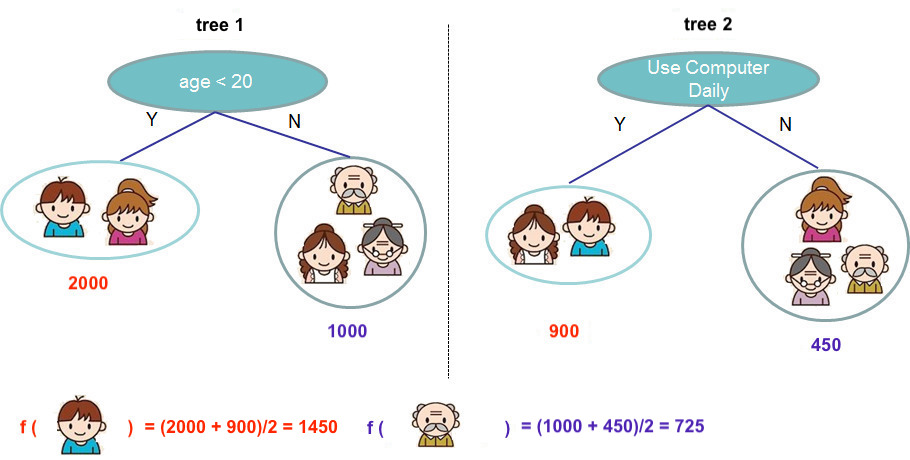
\includegraphics[scale=0.4]{figures/twocart_gboost.jpeg}
              % \\
              % \tiny
              % \url{source: https://xgboost.readthedocs.io/en/latest/tutorials/model.html}
 \end{figure}

\end{frame}
%----------------------------------------------------------------------%
\subsection{Random Forests }
%----------------------------------------------------------------------%
\begin{frame}[fragile]
\frametitle{Random Forests}

\begin{itemize}
  \item Problema con el bagging: si hay un predictor fuerte, diferentes árboles son muy similares entre sí. Si hay alta correlación, ¿está realmente reduciendo la varianza?
\bigskip
\item Bosques (forests): reduce la correlación entre los árboles  en el boostrap.
\bigskip
\item Si hay $p$ predictores, en cada partición use solo  $m <p$ predictores, elegidos al azar.
\bigskip
\item Bagging es forests con $m = p$ (usando todo los predictores en cada partición).
\bigskip
\item Tipicamente $m = \sqrt(p)$
\end{itemize}

\end{frame}

%----------------------------------------------------------------------%
\begin{frame}[fragile]
\frametitle{Ejemplo}
\begin{figure}[H] \centering
  \centering
  
\includegraphics[scale=0.35]{figures/baticomputer_meme.jpg}
  \\
  \tiny photo from \url{https://www.dailydot.com/parsec/batman-1966-labels-tumblr-twitter-vine/}
\end{figure}

\end{frame}


%----------------------------------------------------------------------%
\section{Boosting}
%----------------------------------------------------------------------%
\begin{frame}[fragile]
\frametitle{Boosting: Motivation}

\begin{itemize}
  \item Problema con CART: varianza alta.
  \medskip
   \item Podemos mejorar mucho el rendimiento mediante la agregación 
   \medskip 
   \item El boosting toma esta idea pero lo "encara" de una manera diferente $\rightarrow$ viene de la computación
   \medskip
   \item Va a usar arboles pequeños y a aprender de los errores


\end{itemize}
\end{frame}



%----------------------------------------------------------------------%
\begin{frame}[fragile]
\frametitle{Boosting Trees}


\begin{itemize}
  \item La idea es aprender de los errores lentamente. 
  \medskip
  \item Ajustamos un árbol utilizando los errores del modelo. 
  \medskip
  \item Cada uno de estos árboles puede ser bastante pequeño. 
  \medskip
  \item Esto permite mejorar lentamente aprendiendo $f(.)$ en áreas donde no funciona bien.
  \medskip
  \item OJO: a diferencia de {\it bagging}, la construcción de cada árbol depende en gran medida de los árboles que ya han crecido.
\end{itemize} 
\end{frame}
%----------------------------------------------------------------------%
\begin{frame}[fragile]
\frametitle{Boosting Trees: Algoritmo}

\begin{enumerate}
\item Iniciamos fijando $\hat{f}(x)=0$ y $r_i=y_i$ para todos los $i$ del training set
\medskip
\item Para $m=1,2,...,M$
\begin{enumerate}
  \item Ajustamos un árbol $\hat{f}^m$ con $d$ bifurcaciones ($d+1$ hojas)
  \medskip 
  \item Actualizamos $\hat{f}(x)$ con una versión "shrunken" del nuevo árbol
  \begin{align}
  \hat{f}(x)\leftarrow \hat{f}(x)+\lambda\hat{f}^m(x)
  \end{align}
  \medskip 
  \item Actualizamos los residuales
  \begin{align}
  r_i\leftarrow r_i-\lambda\hat{f}^m(x)
  \end{align}
  \medskip
\end{enumerate}
  \item El modelo final es
  \begin{align}
  \hat{f}_{boost} =\sum_{m=1}^M \lambda \hat{f}^m(x)
  \end{align}
  
\end{enumerate}
\end{frame}
%----------------------------------------------------------------------%
\begin{frame}[fragile]
\frametitle{Example: Default}
\begin{figure}[H] \centering
  \centering
  
\includegraphics[scale=0.35]{figures/baticomputer_meme.jpg}
  \\
  \tiny photo from \url{https://www.dailydot.com/parsec/batman-1966-labels-tumblr-twitter-vine/}
\end{figure}
\end{frame}
%----------------------------------------------------------------------%
\begin{frame}[fragile]
\frametitle{Boosting Trees: Iteraciones}

\begin{itemize}

\item La primer pregunta es sobre cuantas iteraciones (M) usar?
\begin{itemize}
\medskip
  
  \item Cada iteración generalmente reduce el error de ajuste, de modo que para M lo suficientemente grande este error puede hacerse arbitrariamente pequeño (sesgo se va a cero).
  \medskip
  \item Sin embargo, ajustar demasiado bien los datos de entrenamiento puede llevar a overfit (sobreajuste)
  \medskip
  \item Por lo tanto, hay un número óptimo $ M^\star$ que minimiza el error fuera de muestra
  \medskip
  \item Una forma conveniente de encontrar $M^\star$ con validación cruzada

  \end{itemize}
\end{itemize}

\end{frame}

%----------------------------------------------------------------------%
\begin{frame}[fragile]
\frametitle{Boosting Trees: Iteraciones}

\begin{itemize}

\item Los otros hiperparámetros a fijar son
\bigskip
\begin{itemize}
  \item $\lambda$ la tasa a la que aprende, los valores típicos son 0.01 o 0.001
\bigskip
\item El tamaño del árbol. Arboles pequeños (stumps) funcionan bien.
\end{itemize}
\end{itemize}
\end{frame}
%----------------------------------------------------------------------%
\begin{frame}[fragile]
\frametitle{Example: Default}
\begin{figure}[H] \centering
  \centering
  
\includegraphics[scale=0.35]{figures/baticomputer_meme.jpg}
  \\
  \tiny photo from \url{https://www.dailydot.com/parsec/batman-1966-labels-tumblr-twitter-vine/}
\end{figure}


\end{frame}

%----------------------------------------------------------------------%
%----------------------------------------------------------------------%
\end{document}
%----------------------------------------------------------------------%
%----------------------------------------------------------------------%
